% -----------------------------------------------------------------------------
% -----------------------------------------------------------------------------
%  Adaptado de pacote abntex2 http://code.google.com/p/abntex2/
%      por Bruno Eduardo Gomes Barreto
% -----------------------------------------------------------------------------
% -----------------------------------------------------------------------------

\documentclass[
	% -- opções da classe memoir --
	12pt,				% tamanho da fonte
	openright,			% capítulos começam em pág ímpar (insere página vazia caso preciso)
	oneside,	
	a4paper,				% tamanho do papel.
	% -- opções da classe abntex2 --
	%chapter=TITLE,		% títulos de capítulos convertidos em letras maiúsculas
	%section=TITLE,		% títulos de seções convertidos em letras maiúsculas
	%subsection=TITLE,		% títulos de subseções convertidos em letras maiúsculas
	%subsubsection=TITLE,	% títulos de subsubseções convertidos em letras maiúsculas
	% -- opções do pacote babel --
	english,				% idioma adicional para hifenização
	brazil				% o último idioma é o principal do documento
]{abntex2/abntex2} % Entre chaves vai o caminho para o arquivo .cls

%%% Pacotes utilizados %%%
%%% No arquivo meta estão os pacotes e informações relevantes
%%% ao arquivo como nome do autor, orientador, título


% ---
% Pacotes básicos
% ---
\usepackage{bookmark}				% Usa a fonte Bookman Old Style
\usepackage[T1]{fontenc}			% Selecao de codigos de fonte.
\usepackage[utf8]{inputenc}		% Codificacao do documento (conversão automática dos acentos)
\usepackage{color}				% Controle das cores
\usepackage{graphicx}			% Inclusão de gráficos
\usepackage{microtype} 			% para melhorias de justificação

\usepackage[brazilian,hyperpageref]{backref}	 % Paginas com as citações na bibl
\usepackage[alf]{abntex2cite}	% Citações padrão ABNT
\usepackage{float}
\usepackage{url}
\usepackage{enumerate}
\usepackage{siunitx}
\usepackage{setspace}
\usepackage[euler]{textgreek}

%%%%%%%%% NOVO
\usepackage{hyperref}
\hypersetup{
    colorlinks=true,
    linkcolor=blue,
    citecolor=blue,
    filecolor=magenta,      
    urlcolor=blue,
    bookmarksopen=true,
}
\urlstyle{same}

%%%   letra capitular
\usepackage{lettrine}
\usepackage{palatino}

%%%    tabelas - configuração
\usepackage{booktabs}
\usepackage{siunitx}

\usepackage{lscape}


%%% lista de abreviações e siglas automática 
\usepackage{acro}


%%%%%% estilo do capítulo
%%%%%% escolha 1 e tire o comentário
%% acesse a página e escolha
%%http://ctan.math.washington.edu/tex-archive/info/latex-samples/MemoirChapStyles/MemoirChapStyles.pdf

%% primeiro
%\chapterstyle{madsen}

%% segundo
%\chapterstyle{southall}

%% terceiro
%\chapterstyle{Ger}

%% quarto
%\chapterstyle{verville}

%% quinto
\setlength\midchapskip{10pt}
\makechapterstyle{VZ23}{
    \renewcommand\chapternamenum{}
    \renewcommand\printchaptername{}
    \renewcommand\chapnumfont{\Huge\bfseries\centering}
    \renewcommand\chaptitlefont{\Huge\scshape\centering}
    \renewcommand\afterchapternum{%
        \par\nobreak\vskip\midchapskip\hrule\vskip\midchapskip}
    \renewcommand\printchapternonum{%
        \vphantom{\chapnumfont \thechapter}
        \par\nobreak\vskip\midchapskip\hrule\vskip\midchapskip}
}
\chapterstyle{VZ23}

%%%%%%%%%%%%%

\titulo{Painel de Leds escalável com Comunicação SPI}
\autor{José Gualberto Santos Lima \\ Samuel Cardoso da Silva}
\local{Florianópolis - Santa Catarina}
\data{Novembro de 2021}
\instituicao{%
  Instituto Federal de Santa Catarina - IFSC
  \par
  Campus Florianópolis}
\preambulo{Trabalho submetido à avaliação, como requisito parcial, para a obtenção de nota na disciplina de Projeto Integrador, ministrada pelos professores Adriano Regis, Franscisco Edson Nogueira de Melo e Delcino Picinin Junior.}


% Informações do PDF
\makeatletter
\hypersetup{
    	%pagebackref=true,
	pdftitle={\@title}, 
	pdfauthor={\@author},
    	pdfsubject={\imprimirpreambulo},
    pdfcreator={LaTeX with abnTeX2},
	pdfkeywords={abnt}{latex}{abntex}{abntex2}{trabalho acadêmico},
	bookmarksdepth=4
}
\makeatother

% --- 
% Espaçamentos entre linhas e parágrafos 
% --- 

% O tamanho do parágrafo é dado por:
\setlength{\parindent}{1.3cm}

% Controle do espaçamento entre um parágrafo e outro:
%\setlength{\parskip}{0.2cm}  % tente também \onelineskip

%\setbeforesecskip{3em}
%\setbeforesubsecskip{3em}

% ---
% compila o indice
% ---
\makeindex
\usepackage{listings}
\usepackage[utf8]{inputenc}
\usepackage{color}
\usepackage{listingsutf8}

\definecolor{dkgreen}{rgb}{0,0.6,0}
\definecolor{gray}{rgb}{0.5,0.5,0.5}
\definecolor{mauve}{rgb}{0.58,0,0.82}

\lstset{frame=tb,
  aboveskip=3mm,
  belowskip=3mm,
  showstringspaces=false,
  columns=flexible,
  numbers=left,
  numberstyle=\tiny\color{gray},
  keywordstyle=\color{blue},
  commentstyle=\color{dkgreen},
  stringstyle=\color{mauve},
  basicstyle=\ttfamily\footnotesize,
  language=C,
  inputencoding=utf8/latin1
}
\renewcommand{\lstlistingname}{Código}
\renewcommand{\lstlistlistingname}{Lista de \lstlistingname s}


% ---------------------------------------------------
% INICIO DE DOCUMENTO
% ---------------------------------------------------

\begin{document}
%%%%%   comente os capítulos indesejados para que não apareceçam
\noindent

% Seleciona o idioma do documento (conforme pacotes do babel)
%\selectlanguage{english}
\selectlanguage{brazil}

% Retira espaço extra obsoleto entre as frases.
\frenchspacing

% ----------------------------------------------------------
% ELEMENTOS PRÉ-TEXTUAIS
% ----------------------------------------------------------
% \pretextual

% ---
% Capa
% ---
\imprimircapa
% ---

% ---
% Folha de rosto
% (o * indica que haverá a ficha bibliográfica)
% ---
\imprimirfolhaderosto*
% ---

% ---
% Inserir folha de aprovação
% ---

% Isto é um exemplo de Folha de aprovação, elemento obrigatório da NBR
% 14724/2011 (seção 4.2.1.3). Você pode utilizar este modelo até a aprovação
% do trabalho. Após isso, substitua todo o conteúdo deste arquivo por uma
% imagem da página assinada pela banca com o comando abaixo:
%
% \includepdf{folhadeaprovacao_final.pdf}
%


\frontmatter


% ---
% inserir o sumario
% ---


\pdfbookmark[0]{\contentsname}{toc}
\tableofcontents*


\newpage

\listoftables

\newpage

\listoffigures

\cleardoublepage
% ---

\textual
\chapter{Introdução}
% para fazer marcações no texto para eventuais referências, utilize o o label
% variando entre SEC FIG IMAG TAB ALG
\label{sec:introdução}

%para inicializar o primeiro parágrafo de uma seção utilize o padrão a seguir
% onde a letra na chave {A} é a letra em questão que aparecerá 
\lettrine[lines=3]{V}{}ivemos em uma era totalmente digital, onde a informação vem de forma rápida e precisa, o que antes era conhecido apenas por meio da leitura de livros e pesquisa aplicada, hoje, tem-se acesso apenas a distância de um clique. Com isso, não é de se estranhar o acúmulo de informação em meio a cidades e grandes metrópoles, sempre é possível observar letreiros, outdoors, painéis digitais, que normalmente estão sintonizados em alguma propaganda, para promover algo em questão. O dia a dia é frenético nos centros comerciais, então o investimento em tecnologias desse porte no meio dos donos de lojas e estabelecimentos tem se tornado cada vez mais frequente. "O visual é a primeira impressão que temos de um lugar, e a primeira imagem que um cliente tem do seu estabelecimento é a fachada. Por isso, investir em um bom layout para letreiros e fachadas é um diferencial para a divulgação de empresas e  a atração de novos clientes" \cite{SPletras}, tendo em mente toda essa onda dos meios de informação, o grupo decidiu por desenvolver um painel de LEDs, que permitirá o compartilhamento de qualquer tipo de texto por meio de painéis escaláveis, controlado via internet.
 
\section{Contextualização ou definição do problema}
	
Atualmente os painéis e letreiros apresentam configuração através de drivers inbutidos programavéis via computador, uma das metas do projeto é tornar essa configuração mais simples, por meio de uma interface gráfica via internet, a outra meta é tornar o painél escalável, permitindo a junção de dois ou mais painéis para a criação de um maior, sem que isso afete o texto no mesmo.


\section{Objetivos}

O trabalho visa a criação de uma placa de leds escalável com comunicação SPI para que possa haver a expansão da placa,para esse semestre elá será expandida apenas horizontalmente, mas o hardware permitirá a expansão vertical, e a mesma pode ser controlada pelo computador atráves de uma interface gráfica.
		
		\begin{itemize}
			\item Confeccionar uma placa de circuitos impressos (PCI).
			
			\item Criar a interface gráfica que permita ao usuário escolher de forma acessível o que irá aparecer na placa.


		\end{itemize}


% ---
% Capítulo 2
% ---
\chapter{Desenvolvimento}


\lettrine[lines=3]{P}{} artindo da utilização de boa parte do projeto efetuado em semestres anteriores, busca-se melhorar todo o funcionamento da placa, tornando-a modular e totalmente programável. Para controlar o que aparecerá no painél, será utilizada uma junção de dois CIs, o 74hc595 e o 74hc138, que receberão a mensagem via ESP32, responsável por fazer a conexão da interface gráfica ate os CIs. O 74hc595 será utilizado como escravo na comunicação SPI. Serial Peripheral Interface ou SPI é um protocolo que permite a comunicação do microcontrolador com diversos outros componentes, formando uma rede. É uma especificação de interface de comunicação série síncrona usada para comunicação de curta distância, principalmente em sistemas embarcados. Dessa forma, o sinal é enviado para todos os LEDs a partir de só um microcontrolador. Já o 74hc198 transmite o sinal para o LED que precisa ser ligado. 

O projeto passará por testes no software Proteus, onde serão analisadas questões como o comportamento de alguns componentes, e também o funcionamento da programação em meio a utilização do circuito e após isso será iniciada a fase de desenvolvimento da PCI. Com relação a programação, serão utilizados dois tipos de linguagem, "C++" para a ESP32 e "python" pra o software Glade, onde será desenvolvida a interface gráfica que permitira a edição dos textos do painél.

Abaixo podemos ver algumas figuras do projeto de semestres passados, que mostram os esquemáticos no proteus(figura \ref{fig:PCB}), e módulo de LEDs(figura \ref{fig:modulo}) .


		\begin{figure}[H]
			\centering\footnotesize
			\caption{PCB e esquema no Proteus}
			\begin{center}
			    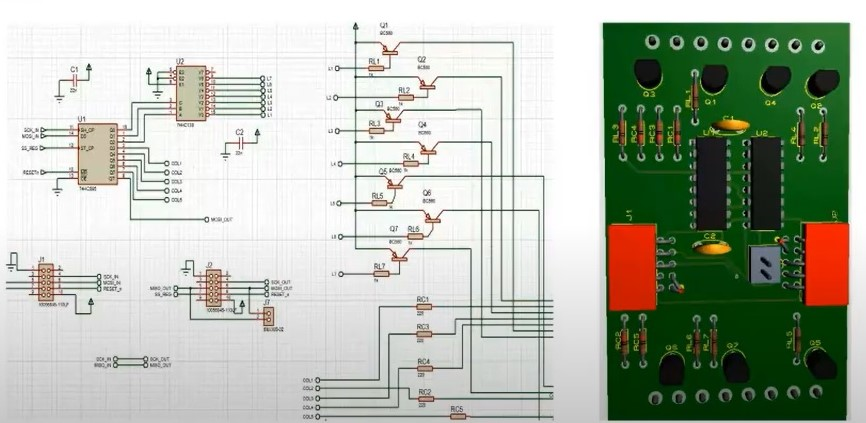
\includegraphics[scale=0.7]{imagens/PCP.jpg}
			\end{center}
			\label{fig:PCB}
			\par Fonte: Arthur Loss, Ivan Correa, Marcelo Junges, Fernanda Brizdo.
		\end{figure}
		\begin{figure}[H]
			\centering\footnotesize
			\caption{Módulos}
			\begin{center}
			    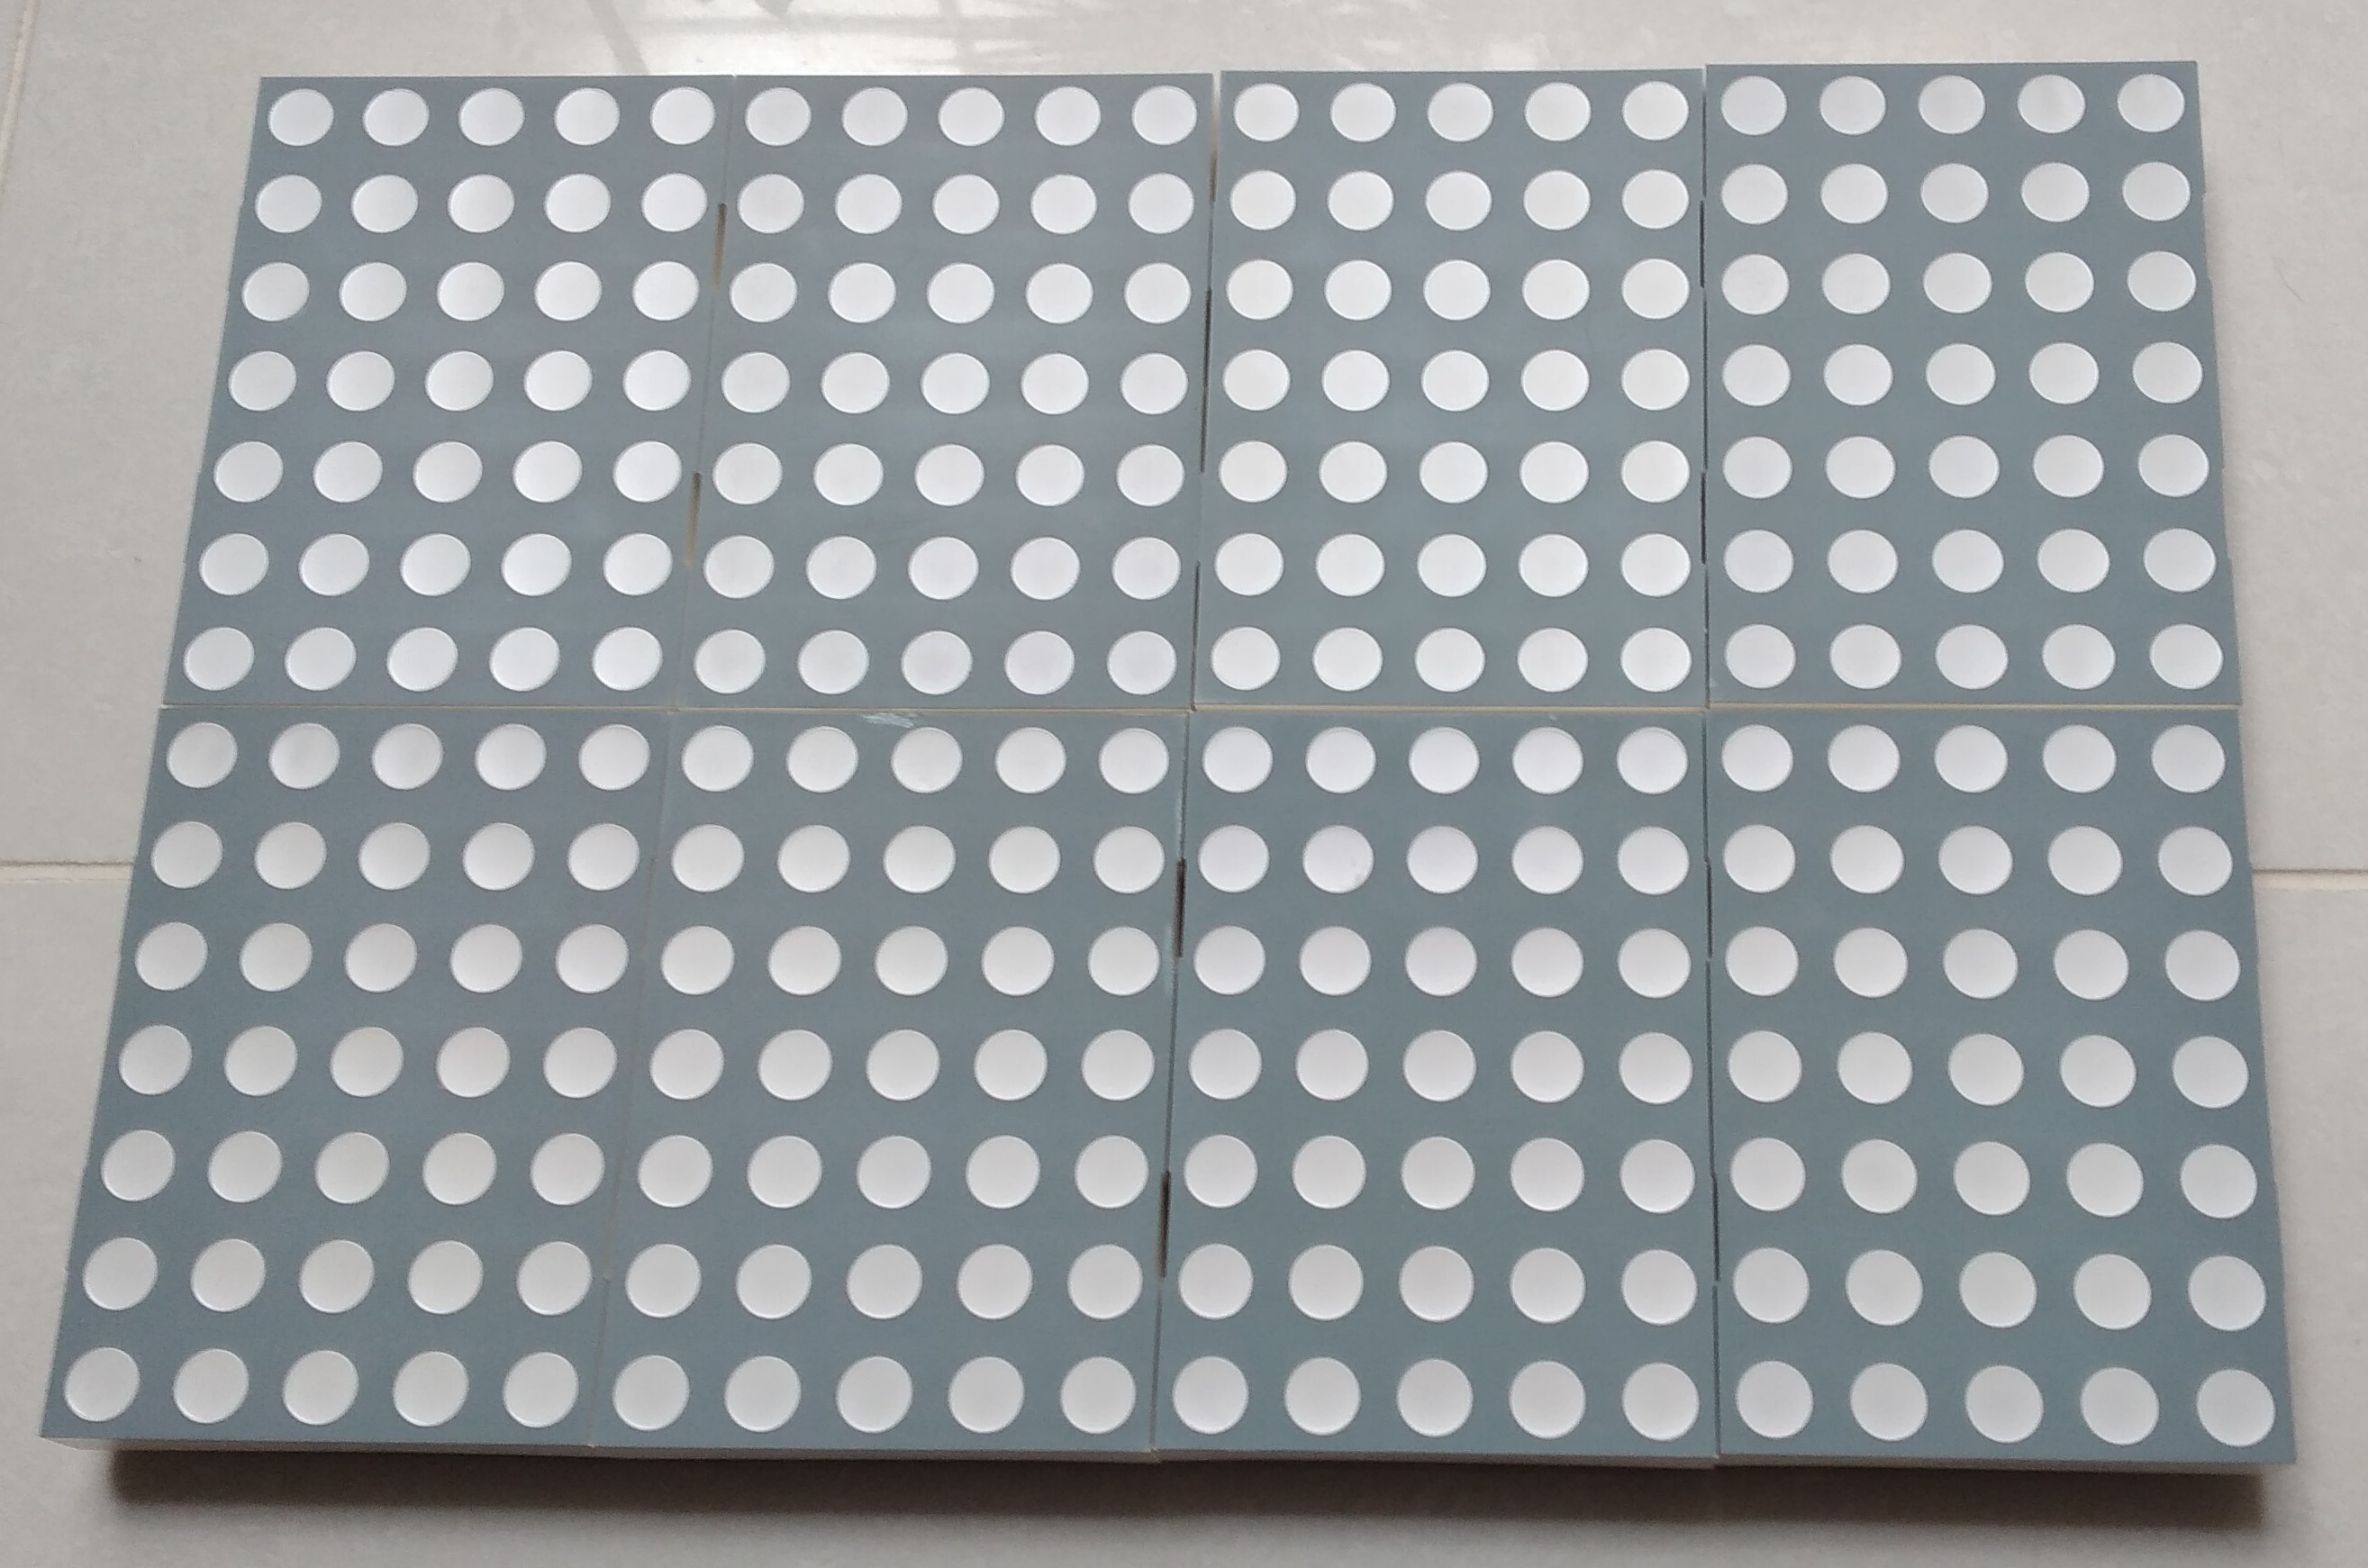
\includegraphics[scale=0.1]{imagens/20210812_111039.jpg}
			\end{center}
			\label{fig:modulo}
			\par Fonte: Edson Melo
		\end{figure}

\section{Itens a serem Adquiridos}

Os componentes implementados no projeto, estão apresentados na Tabela \ref{table:Componentes do projeto}.

\begin{table}[H]
	\centering\footnotesize
	\caption{ Componentes do Projeto Mercado Livre}	
	\begin{tabular}{p{5cm}S[table-format=0.2]S[table-format=0.2]S[table-format=0.2]S[table-format=0.2]S[table-format=0.2]S[table-format=0.2]S[table-format=0.2]}
		\toprule	
		Componentes & {Qtd necessaria} & {Qtd} & {Preço}  & {Link}
		\\
		\midrule
		Módulos de leds & {6} & {10} & {40,50} & \cite{Modulos}\\ 
		BC547 & {42} & {50} & {18,99} & \cite{BC547}\\
		74hc595 & {6} & {10} &{23,74} & \cite{74hc595}\\
		74hc138 & {6} & {10} & {25,42} &\cite{74hc138}\\
		Capacitor 100 nF & {12} & {100} & {28,84}  & \cite{Capacitor100nF}\\
		Conector header 16 pinos 90º & {12} & {10} & {18,90} & \cite{Conectorheader16Pinos}\\
		Conector Latch Fêmea 10 Vias & {12} & {50} & {37,99} & \cite{Conectorlatchfemea}\\ 
		Cabo fita  & {1.27mm/m} & {1} & {18,90} &\cite{CaboFita}\\ 
		Fonte de 5 V 5 A  & {1} & {1} & {32,50} & \cite{Fonte5v}\\
		Esp 32  & {1} & {1} & {42,20} & \cite{Esp32}\\
		Resistores 330 ohms & {42} & {100} & {12,69} & \cite{330}\\
		Resistores 1k ohms & {30} & {100} & {12,49} & \cite{1k}\\
		\bottomrule
	\end{tabular}
	\label{table:Componentes do projeto}
	\par Fonte: Elaborado pelo próprio autor
\end{table}

Também fizemos uma lista em outro site, apresentando valores mais baratos para compra, que estão presentes na tabela abaixo:


\begin{table}[H]
	\centering\footnotesize
	\caption{ Componentes do Projeto Báu da eletrônica}	
	\begin{tabular}{p{5cm}S[table-format=0.2]S[table-format=0.2]S[table-format=0.2]S[table-format=0.2]S[table-format=0.2]S[table-format=0.2]S[table-format=0.2]}
		\toprule	
	Componentes & {Qtd necessaria} & {Qtd} & {Preço}  & {Link}
		\\
		\midrule
		BC547 & {42} & {42} & {15,96} &  \cite{BC547novo}\\
		74hc595 &  {6} & {6} & {13,08} &  \cite{74hc595novo}\\
		74hc138 &  {6} & {6} & {18,42} & \cite{74hc138novo}\\
		Capacitor 100 nF & {12} & {12} & {1,56} & \cite{Capacitor100nFnovo}\\
		Conector header 16 pinos 90º & {12} & {12}& {21,72} &  \cite{Conectorheader16Pinosnovo}\\
		Conector Latch Fêmea 10 Vias & {12} & {12} & {9,36} &  \cite{Conectorlatchfemeanovo}\\ 
		Cabo fita  & {1.27mm/m} & {1} & {4,25} &\cite{CaboFitanovo}\\ 
		Esp 32  & {1} & {1} & {87,40} &  \cite{Esp32novo}\\
		Resistores 330 ohms & {42} & {42} & {2,52} &  \cite{330novo}\\
		Resistores 1k ohms & {30} & {30} & {1,80} & \cite{1knovo}\\
		\bottomrule
	\end{tabular}
	\label{table:Componentes do projeto}
	\par Fonte: Elaborado pelo próprio autor
\end{table}

É importante salientar que alguns componentes como módulo de LEDs, Esp32, cabo fita e resistores, poderão ser providenciados pelo IFSC em conjunto com os professores orientadores. 

\chapter{Cronograma}

O cronograma apresentado na Tabela \ref{table:cronogramaT1} detalha as atividades a serem executadas entre os encontros 8 e 22, exclusivamente, e compreende uma divisão semanal.

\begin{table}[H]
	\centering\footnotesize
	\caption{Cronograma.}	
	\begin{tabular}{p{10cm}S[table-format=0.5]S[table-format=0.5]S[table-format=0.5]S[table-format=0.5]S[table-format=0.2]S[table-format=0.2]S[table-format=0.2]}
		\toprule	
		{Semanas:} & {1} & {2} & {3} & {4} & {5} & {6} & {7}\\
		\midrule
		
		Programar interface gráfica em python(Glade)  &  & X & X &  &  &  &  \\
		Estudo sobre os CIs &  &  & X & X &  &  &\\
		Teste da comunicação SPI    &  &  &  &  & X & X &  \\ 
		Enviar mensagens estáticas no modulo de LEDs   &  &  &  &  &  & X & X \\
		Montagem em matriz de contato & & & & & & & X\\
		\bottomrule
	\end{tabular}
	\label{table:cronogramaT1}
	\par Fonte: Elaborado pelo próprio autor
\end{table}		
\chapter{Considerações Finais}

O presente trabalho tem como objetivo a produção de uma placa de LEDs escalável que pode ser expandida a gosto do usuário e pode ser controlada a partir de uma interface gráfica. Esse projeto, pretende facilitar a passagem de informações no comércio de maneira acessível. Com o projeto foi adquirido conhecimentos sobre eletrônica analógica,
eletrônica digital, programação e como integrá-las.

%referencias



% ----------------------------------------------------------
% ELEMENTOS PÓS-TEXTUAIS
% ----------------------------------------------------------
\postextual
\Spacing{1.5}
% -----------------------------------------------------------------------------
% Referencias Bibliograficas
% -----------------------------------------------------------------------------
\bibliography{referencias}

% ----------------------------------------------------------
% Apêndices
% ----------------------------------------------------------

%% ---
% Inicia os apêndices
% ---
\begin{apendicesenv}
    
    % ----------------------------------------------------------
    \chapter{Primeiro apêndice}
    % ----------------------------------------------------------
    
    Os apêndices são textos ou documentos elaborados pelo autor, a fim de complementar sua argumentação, sem prejuízo da unidade nuclear do trabalho.
    
\end{apendicesenv}
%% Anexos
% ----------------------------------------------------------

% ---
% Inicia os anexos
% ---
\begin{anexosenv}

% ---
\chapter{Primeiro anexo.}
% ---

Os anexos são textos ou documentos não elaborados pelo autor, que servem de fundamentação, comprovação e ilustração.

\end{anexosenv}

\end{document}